%%  File: main.tex
%%  Author: Matthew Gidden
%%  Created: Sept. 17, 2013
%%  Purpose: Prelim Presenation
     
\documentclass[10pt]{beamer}
\usetheme[white]{Wisconsin}
%\title[short title]{long title}
\title[Cyclus]{An Agent-Based Framework for Fuel Cycle Simulation with
  Recycling}
%\subtitle[short subtitle]{long subtitle}
%\author[short name]{long name}
\author[MJG]{Matthew Gidden}
%\date[short date]{long date}
\date[10.03.2013]{GLOBAL13 \\ October 03, 2013}
%\institution[short name]{long name}
\institute[UW-Madison]{University of Wisconsin-Madison}
% Page numbers.
\setbeamertemplate{footline}[page number]
% Those icons  in the references are terrible looking.
\setbeamertemplate{bibliography item}[text]
%try to get rid of header on title page\dots
\makeatletter
    \newenvironment{withoutheadline}{
        \setbeamertemplate{headline}[default]
        \def\beamer@entrycode{\vspace*{-\headheight}}
    }{}
\makeatother

% packages
\usepackage{multirow} % combining rows in tables
%\usepackage{footnote}

%% % this is a great way to compile only one (or more) frames at a time as you're
%% % working, saving tons on compile time
%% \includeonlyframes{current}

\begin{document}
%%%%%%%%%%%%%%%%%%%%%%%%%%%%%%%%%%%%%%%%%%%%%%%%%%%%%%%%%%%%%
%% From uw-beamer Here's a handy bit of code to place at 
%% the beginning of your presentation (after \begin{document}):
\newcommand*{\alphabet}{ABCDEFGHIJKLMNOPQRSTUVWXYZabcdefghijklmnopqrstuvwxyz}
\newlength{\highlightheight}
\newlength{\highlightdepth}
\newlength{\highlightmargin}
\setlength{\highlightmargin}{2pt}
\settoheight{\highlightheight}{\alphabet}
\settodepth{\highlightdepth}{\alphabet}
\addtolength{\highlightheight}{\highlightmargin}
\addtolength{\highlightdepth}{\highlightmargin}
\addtolength{\highlightheight}{\highlightdepth}
\newcommand*{\Highlight}{\rlap{\textcolor{HighlightBackground}{\rule[-\highlightdepth]{\linewidth}{\highlightheight}}}}
%%%%%%%%%%%%%%%%%%%%%%%%%%%%%%%%%%%%%%%%%%%%%%%%%%%%%%%%%%%%%

%% Cyclus/MJG Custom Commands
\newcommand{\Cyclus}{\textsc{Cyclus} }
%%%%%%%%%%%%%%%%%%%%%%%%%%%%%%%%%%%%%%%%%%%%%%%%%%%%%%%%%%%%%

%%--------------------------------%%
\begin{withoutheadline}
\frame{
  \titlepage
}
\end{withoutheadline}

%%--------------------------------%%
%% \AtBeginSection[]{
%% \begin{frame}
%%   \frametitle{Outline}
%%   \tableofcontents[currentsection]
%% \end{frame}
%% }
%---------------||||

%---------------||||
\section{Introduction}

\begin{frame}[ctb!]
  \frametitle{\Cyclus}
  
\end{frame}

\begin{frame}[ctb!]
  \frametitle{Motivating Question}
  
  \begin{block}{Dynamic Resource Exchange}
    If facilities are treated as individual black boxes and connections between
    facilities are determined dynamically, how does one match suppliers with
    demanders considering supply constraints and, supply response to
    quality-based demands, and issues of fungibility?
  \end{block}

\end{frame}

\section{Background}
\subsection{Fuel Cycle Simulators}

Previous implementations of fuel cycle simulators have varied both in
methodology and distribution platform. The general purpose of all simulators is
to model the flow of material around the fuel cycle in order to determine the
viability of various proposed fuel cycles and their relative
performance \textit{vis-a-vis} a variety of metrics including resource
utilization, costs, and proliferation resistance. However, there are a few key
choices that have been historically made by all simulation developers,
including: what program or language to use, how to determine the flow of
material when there are competing sources or sinks for that material, how to
determine which facilities to build and when to build them, and at what level of
fidelity simulation physics should be modeled (e.g., should material decay or
should it not). One could describe these are the major design choices for
simulation development teams to assess, and in general approaches are taken
which span the gamut from the computationally ``easy'' to the computationally
``complex'' and the spectrum of almost full user-control to more substantial use
of automated decision making.



\subsection{Agent Based Supply Chain Simulation}

There are a number of agent-based supply chain frameworks and implementations
available in the literature with varying levels of accessibility due to
proprietary
considerations \cite{swaminathan_modeling_1998,julka_agent-based_2002,van_der_zee_modeling_2005,chatfield_multi-formalism_2007}.
However, the nuclear fuel cycle presents a few unique characteristics not
explicitly treated in the literature. Perhaps the most difficult consideration
we have identified is the need to specify target fuel recipes and match
suppliers and consumers based on the requested recipe, i.e.  there are both
quantity and quality constraints placed on a requested commodity. An additional
difficulty arises with the enforcement of regional-boundary constraints
(e.g. prohibiting HEU trade between regions) and inter-enterprise
preferences. We propose to tackle both issues via a comprehensive supply/demand
matching mechanism.

We propose using a supply/demand matching algorithm that is comprised 
of three main procedures: request-for-bids, preference assignment, 
and resolution. The request-for-bids step signals the producers of 
various commodities of the demand and material specification for 
those commodities. The preference assignment step allows the customers
to analyze each bid in order to assign a preference. The managers of 
these customers (be they at the region or enterprise level) are 
allowed to affect the decision making process at this point in order 
to inform the preferences of the customers covered by their policy 
space. The resolution step takes the as input the bids and 
preferences and outputs the material flows for the given time step.\cite{cyclus2012}

\subsection{Mathematical Programming}

\section{Methodology}

\begin{frame}[ctb!]
  \frametitle{Resource Exchange Generality}

  To determine a supply-demand resource exchange for \textit{general} facilities
  in the fuel cycle, information about both the supply and demand must be known.

  \vspace{0.2cm}
  
  For example:
  \begin{itemize}
    \item enrichment facilities - production constraints
    \item reactors - fuel requests
    \item fabrication facilities - fuel supply
  \end{itemize}
  
\end{frame}

\begin{frame}[ctb!]
  \frametitle{Resource Exchange Generality}

  \begin{figure}
    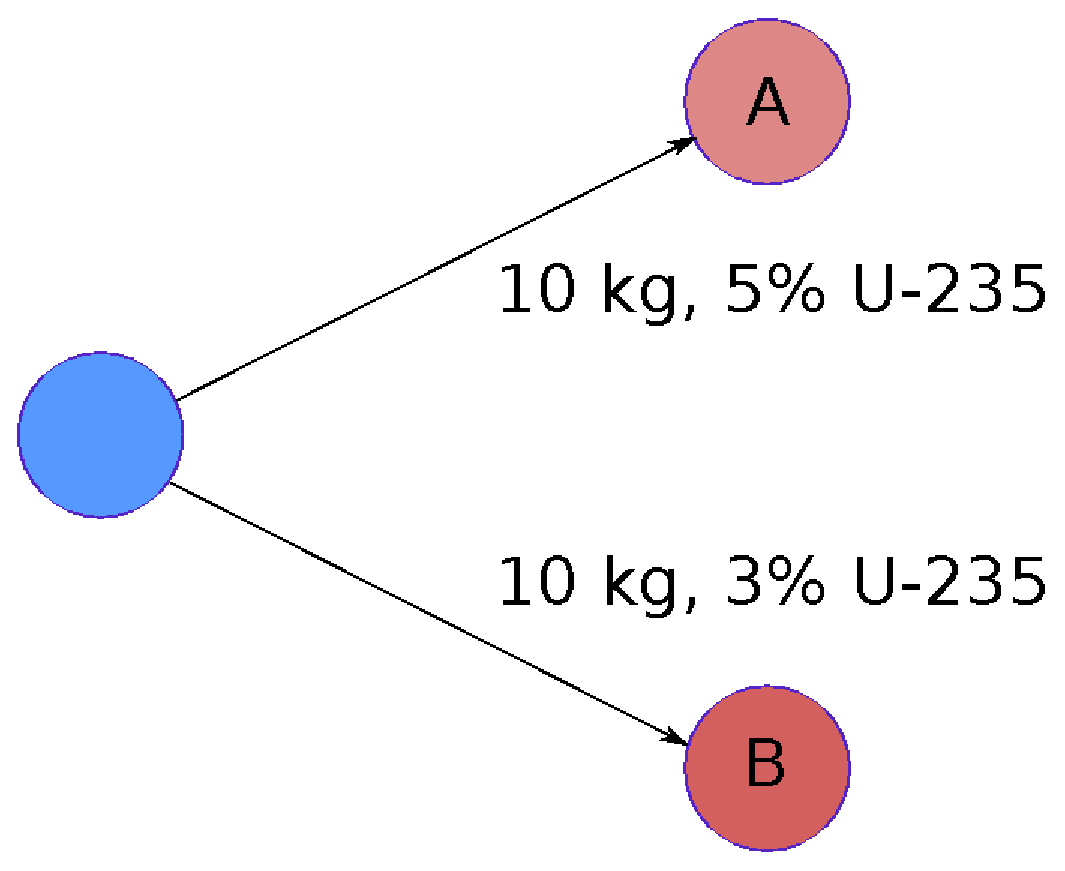
\includegraphics[height=3cm]{./images/enr.eps}
    \caption{Two Demands for Enriched Uranium}
  \end{figure}
  
  \begin{table} [h!]
    \begin{tabular}{|c|c|c|}
      \hline  
      Order & SWU & Nat'l U (kg) \\
      \hline  
      A & 71 & 112\\
      B & 34 & 64\\
      \hline  
    \end{tabular}
  \end{table}

\end{frame}

\begin{frame}[ctb!]
  \frametitle{Resource Exchange Generality}

  This proposal generalizes the exchange of resources in two steps:

  \begin{enumerate}
    \item Gather the information required to make a material flow decision
    \item Solve for material flow
  \end{enumerate}
\end{frame}

\begin{frame}[ctb!]
  \frametitle{Resource Exchange Information Gathering}

  Inspiration taken from Julka et. al. \cite{julka_agent-based_2002},

  \begin{itemize}
    \item fuel cycle is a supply chain
    \item individual facilities are agents
    \item petroleum industry also deals with material quality
  \end{itemize}
  
\end{frame}

\begin{frame}[ctb!]
  \frametitle{Resource Exchange: Request for Bids}
  \begin{figure}
    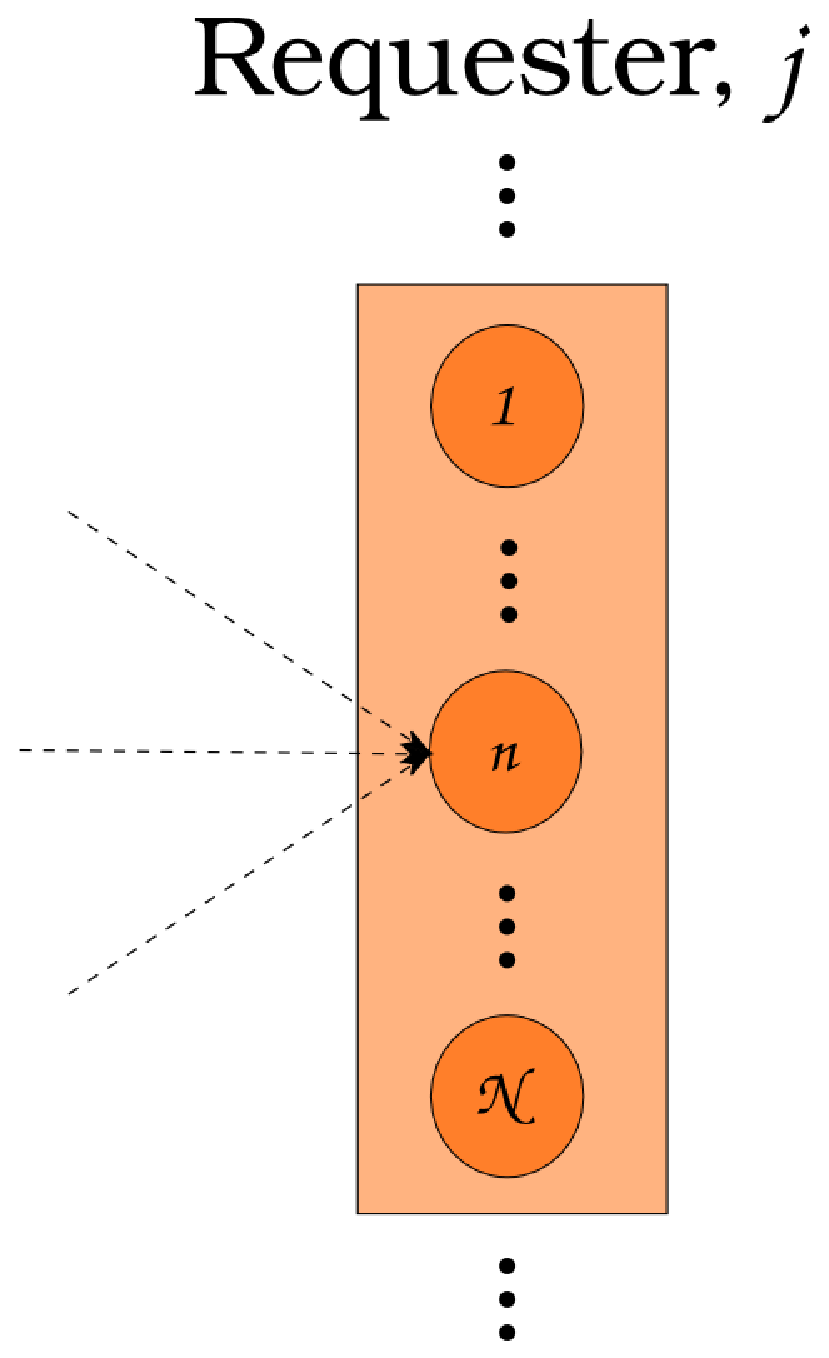
\includegraphics[height=5cm]{./images/requester.eps}
    \caption{Consumers define their demand for commodities during the Request
      for Bids (RFB) phase.}
  \end{figure}
\end{frame}

\begin{frame}[ctb!]
  \frametitle{Resource Exchange: Response to Request for Bids}
  \begin{figure}
    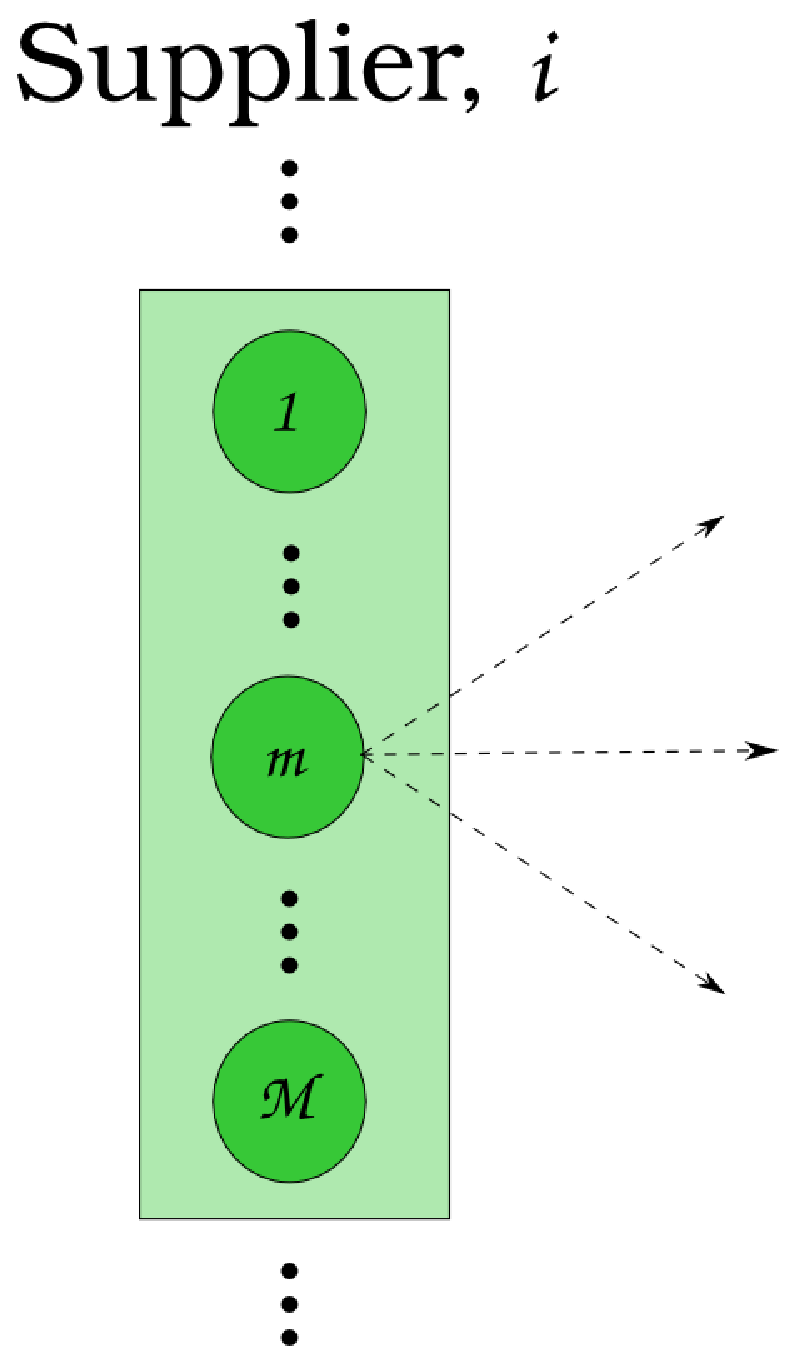
\includegraphics[height=5cm]{./images/supplier.eps}
    \caption{Suppliers respond to each request during the Response to Request
      for Bids (RRFB) phase.}
  \end{figure}
\end{frame}

\begin{frame}[ctb!]
  \frametitle{Resource Exchange: Preference Adjustment}
  \begin{figure}
    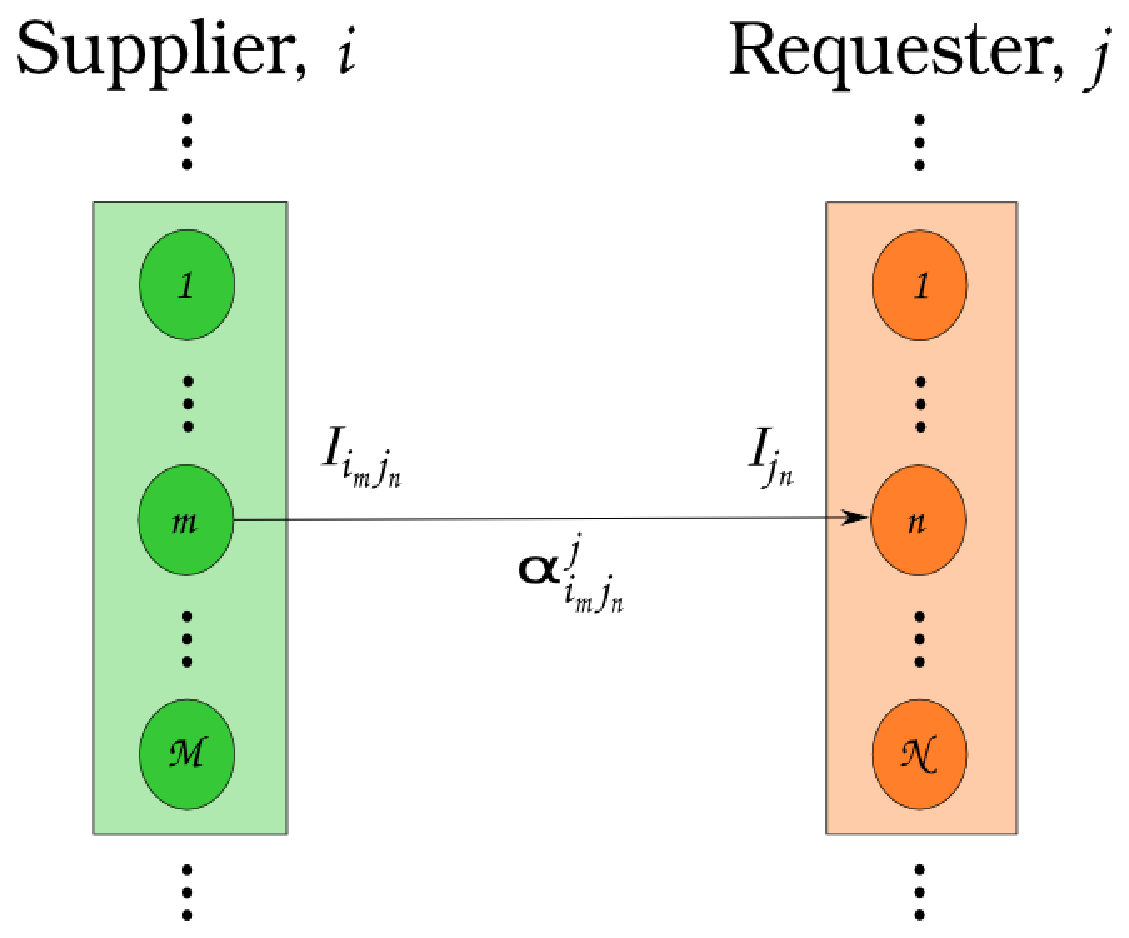
\includegraphics[height=4cm]{./images/supplier-requester.eps}
    \caption{Consumers adjust preferences based on Supplier-given information
      during the Preference Adjustment (PA) phase.}
  \end{figure}

  Managers of facilities (institutions, regions) are then allowed to perturb
  preferences.
\end{frame}

\begin{frame}[ctb!]
  \frametitle{Resource Exchange: Full Picture}
  \begin{figure}
    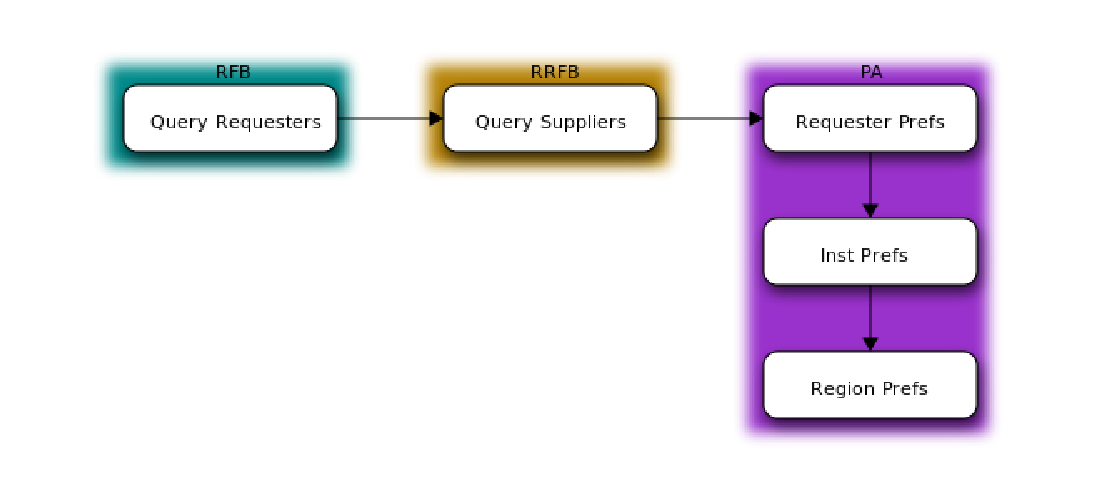
\includegraphics[height=5cm]{./images/exchange.eps}
    \caption{A flow chart of the information gathering phases.}
  \end{figure}
\end{frame}

\begin{frame}[ctb!]
  \frametitle{Resource Exchange Solution Mechanism}

  A Multicommodity Transportation Problem (MTP) formulation naturally fits the
  requirements of the simulation.

  \begin{itemize}
    \item supplier and consumer facilities
    \item discrete transfers of commodities
    \item demand can be met by multiple commodities
  \end{itemize}

  Departs from classic MTP, thus is called Generic Fuel Cycle Transportation
  Problem (GFCTP).
  
\end{frame}

\begin{frame}[ctb!]
  \frametitle{GFCTP - Overview}
  
  The Generic Fuel Cycle Transportation problem assumes the following:
  \begin{itemize}
    \item there is a set of suppliers, a set of requesters, a set of
      commodities, and a set of possible resource transfers, defining arcs
      between suppliers and requesters
    \item a cardinal preference ordering is defined over the set of possible
      resource transfers
    \item suppliers can be constrained both by resource quantities and qualities
    \item multiple commodity types may satisfy a consumer
  \end{itemize}

  A linear programming (LP) formulation and mixed integer-linear programming
  (MILP) formulation is proposed.

\end{frame}
  

\begin{frame}[ctb!]
  \frametitle{GFCTP - Nomenclature}

  Nomenclature used:
  \begin{itemize}
    \item set of commodities, $H$
    \item set of suppliers, $I$
    \item set of requesters, $J$
    \item flow, $x^h_{i,j}$
  \end{itemize}

\end{frame}

\begin{frame}[ctb!]
  \frametitle{GFCTP (LP) - Request Constraint}
  
  Requests
  \begin{itemize}
    \item can be met by multiple commodities, e.g., UOX and MOX
    \item are comprised of
      \begin{itemize}
        \item a quantity, $d_j$
        \item a set of commodities, $H_j$
      \end{itemize}
  \end{itemize}

  \begin{equation}
    \sum_{i \in I}\sum_{h \in H_{j}} x_{i,j}^{h} \geq d_{j}(H_{j})  \: \forall j \in J
  \end{equation}
  
  Feasibility can be guaranteed by using ``fake'' supplier with negative
  preference or infinite cost.

\end{frame}

\begin{frame}[ctb!]
  \frametitle{GFCTP (LP) - Supply Constraint - Example}

  Supply
  \begin{itemize}
    \item can have multiple possible constraints
    \item constraints can be functions of quality and quantity
  \end{itemize}

  E.g., an enrichment facility that provides the commodity enriched uranium (ER):
  \begin{itemize}
    \item A processing constraint, which has units of SWU
    \item An inventory constraint, which has units of kilograms of natural
      uranium (NU)
  \end{itemize}

\end{frame}

\begin{frame}[ctb!]
  \frametitle{GFCTP (LP) - Supply Constraint - Example}
  
  Given
  \begin{itemize}
    \item a requested enrichment level, $\varepsilon_j$
    \item a supply capacity, $s$
    \item a conversion function, $f$
  \end{itemize}

  Associated constraints are
  \begin{equation}
    \sum_{j \in J} f_{SWU}(\varepsilon_j) x_{i,j}^{EU} \leq s_{i,SWU} 
  \end{equation}

  \begin{equation}
    \sum_{j \in J} f_{NU}(\varepsilon_j) x_{i,j}^{EU} \leq s_{i,NU} 
  \end{equation}

  \pause

  These constraints are a function of the isotopic profile of the request, or
  \textit{quality}, $q_j$. More generally suppliers may have conversion
  functions, which are functions of the request quality,
  $\beta_{i,k}(q_{j}^{h})$.

\end{frame}

\begin{frame}[ctb!]
  \frametitle{GFCTP (LP) - Supply Constraint}

  Associated constraints are
  \begin{equation}
    \sum_{j \in J}\beta_{i,k}(q_{j}^{h}) x_{i,j}^{h} \leq s_{i,k} 
    \: \forall \: k \in K_{i}^{h},  
    \forall \: i \in I, \forall \: h \in H
  \end{equation}

  with notation defined as
  \begin{itemize}
    \item $h$ - a commodity
    \item $K_i^h$ - a set of constraints
    \item $s_{i,k}$ - a supply capacity
    \item $\beta_{i,k}(q_{j}^{h})$ - a conversion function
  \end{itemize}

\end{frame}

\begin{frame}[ctb!]
  \frametitle{GFCTP (LP) - Objective Function}

  Two options in proposed framework:
  \begin{enumerate}
    \item maximize preferences
    \item minimize cost
  \end{enumerate}

  Pros and cons:
  \begin{itemize}
    \item preferences are ``natural'' fit
    \item economics is a future concern
    \item cost minimization requires a translation function
  \end{itemize}

\end{frame}

\begin{frame}[ctb!]
  \frametitle{GFCTP (LP) - Objective Function}

  Assuming there is such a function, $f$, i.e.,
  \begin{equation}
    f : \alpha_{i,j}(h) \to c_{i,j}^{h}
  \end{equation}

  The the objective function is
  \begin{equation}
    \min \sum_{h \in H}\sum_{i \in I}\sum_{j \in J}c_{i,j}^{h} x_{i,j}^{h} 
  \end{equation}

\end{frame}

\begin{frame}[ctb!]
  \frametitle{GFCTP (LP) - Formulation} 

  With the normal non-negative flow constraint, the full GFCTP formulation is:
  
  %%%
  \begin{subequations}\label{eqs:GFCTP-LP}
    \begin{align}
      %%
      \min_{z} \:\: & 
      z = \sum_{h \in H}\sum_{i \in I}\sum_{j \in J}c_{i,j}^{h} x_{i,j}^{h} 
      & \label{eqs:GFCTP-LP_obj} \\
      %%
      \text{s.t.} \:\: &
      \sum_{j \in J}\beta_{i,k}(q_{j}^{h}) x_{i,j}^{h} \leq s_{i,k} 
      &
      \: \forall \: k \in K_{i}^{h},  
      \forall \: i \in I, \forall \: h \in H \label{eqs:GFCTP-LP_sup} \\
      %%
      &
      \sum_{i \in I}\sum_{h \in H_{j}} x_{i,j}^{h} \geq d_{j}(H_{j}) 
      & 
      \forall \: j \in J \label{eqs:GFCTP-LP_dem} \\
      %%
      &
      x^h_{i,j} \geq 0
      &
      \forall \: x \in X \label{eqs:GFCTP-LP_x}
      %%
    \end{align}
  \end{subequations}
  %%% 
\end{frame}

\begin{frame}[ctb!]
  \frametitle{GFCTP (LP) - Comments} 
  
  Issues with LP formulation:
  \begin{enumerate}
    \item orders can be split
    \item orders can be satisfied by multiple suppliers
  \end{enumerate}

  Consider a thermal reactor's order constraint for UOX and MOX under the LP
  framework:
  \begin{equation}
    \sum_{i \in I} x_{i}^{MOX} + x_{i}^{UOX} \geq d(\{MOX,UOX\})
  \end{equation} 

  Given a solution, $x^{MOX}$, and $x^{UOX}$, the following values are possible:
  \begin{equation}
    x^{MOX} \in [0, d(\{MOX,UOX\})], \: x^{UOX} \in [0, d(\{MOX,UOX\})]
  \end{equation} 

\end{frame}

\begin{frame}[ctb!]
  \frametitle{GFCTP (MILP) - Overview}

  Split consumers into two groups:
  \begin{enumerate}
    \item those that require \textit{exclusive} orders
    \item those allow \textit{partial} orders
  \end{enumerate}

  \begin{equation}\label{eqs:consumer-union}
    J = J_{p} \cup J_{e}
  \end{equation}

  Introduce a binary variable, $y_{i,j}^{h}$.  
  \begin{itemize}
    \item 1 if consumer $j$ is sent commodity $h$ by supplier $i$
    \item restrict sum of variables for consumer $j$ to 1
  \end{itemize}

  \begin{equation}
    \sum_{h \in H_j}\sum_{i \in I}  y_{i,j}^{h} = 1
     \: \forall \: j \in J_{e}
  \end{equation}
  
\end{frame}

\begin{frame}[ctb!]
  \frametitle{GFCTP (MILP) - Request Constraint} 

  There are now two requests constraints, for each family of requests:

  \begin{equation}
    \sum_{i \in I}\sum_{h \in H_{j}} x_{i,j}^{h} \geq d_{j}(H_{j})
     \: \forall \: j \in J_{p}
  \end{equation}
  
  \begin{equation}    
    \sum_{i \in I}\sum_{h \in H_{j}} y_{i,j}^{h} \tilde{x}_{j}^{h} \geq d_{j}(H_{j}) 
     \: \forall \: j \in J_{e}
  \end{equation}

  The combination $y_{i,j}^{h} \tilde{x}_{j}^{h}$ is equivalent to the flow of
  commodity $h$ from supplier $i$ to requester $j$, $x^h_{i,j}$.
\end{frame}

\begin{frame}[ctb!]
  \frametitle{GFCTP (MILP) - Supply Constraint} 

  Supply constraints also incorporate to two possible flows of material out of a
  supplier:
  
  \begin{equation}    
    \sum_{j \in J_{p}}\beta_{i,k}(q_{j}^{h}) x_{i,j}^{h}
    + \sum_{j \in J_{e}}\beta_{i,k}(q_{j}^{h}) y_{i,j}^{h} \tilde{x}_{j}^{h} \leq s_{i,k}^{h}
     \: \forall \: i \in I, \: \forall \: k \in K_{i}^{h}, \forall \: {h \in H}
  \end{equation}
  
\end{frame}

\begin{frame}[ctb!]
  \frametitle{GFCTP (MILP) - Formulation} 
  
  With a similar treatment of the objective function, the full formulation is:

  \fontsize{7pt}{\baselineskip}\selectfont  
  \begin{subequations}\label{eqs:GFCTP-E}
    \begin{align}
      %%
      \label{eq:GRCTP-E_obj}
      \min_{z} \:\: 
      & 
      z = \sum_{h \in H}\sum_{i \in I}\sum_{j \in J_{p}}c_{i,j}^{h} x_{i,j}^{h} 
      + \sum_{h \in H}\sum_{i \in I}\sum_{j \in J_{e}}c_{i,j}^{h} y_{i,j}^{h} \tilde{x}_{j}^{h}
      && \\
      %%
      \label{eq:GRCTP-E_sup}
      &
      \text{s.t.} \:\: 
      \sum_{j \in J_{p}}\beta_{i,k}(q_{j}^{h}) x_{i,j}^{h}
      + \sum_{j \in J_{e}}\beta_{i,k}(q_{j}^{h}) y_{i,j}^{h} \tilde{x}_{j}^{h} \leq s_{i,k}^{h} \nonumber \\
      &
      \qquad\qquad\qquad\qquad
      \forall \: i \in I, \: \forall \: k \in K_{i}^{h}, \forall \: {h \in H}\\
      %%
      \label{eq:GRCTP-E_dem_p}
      &
      \sum_{i \in I}\sum_{h \in H_{j}} x_{i,j}^{h} \geq d_{j}(H_{j})
      &
      \forall \: j \in J_{p} &\\
      %%
      \label{eq:GRCTP-E_dem_e}
      &
      \sum_{i \in I}\sum_{h \in H_{j}} y_{i,j}^{h} \tilde{x}_{j}^{h} \geq d_{j}(H_{j}) 
      &
      \forall \: j \in J_{e}  &\\
      %%
      \label{eq:GRCTP-E_sumy}
      &
      \sum_{h \in H}\sum_{i \in I} y_{i,j}^{h} = 1
      &
      \forall \: j \in J_{e}  &\\
      %%
      \label{eq:GRCTP-E_x}
      &
      x_{i,j}^{h} \geq 0
      &
      \forall \: x \in X  &\\
      %%
      \label{eq:GRCTP-E_y}
      &
      y_{i,j}^{h} \in \{0,1\}
      &
      \forall \: y \in Y &
      %%
    \end{align}
  \end{subequations}

\end{frame}

\begin{frame}[ctb!]
  \frametitle{Next Steps} 
  
  \begin{itemize}
    \item all work will be done in the
      \href{github.com/cyclus/cyclus}{\Cyclus} code base, incorporating
      continuous integration and unit testing
    \item the \Cyclus team has identified the one and two-tier fuel cycles
      proposed in the recent Dynamic Systems Analysis Report for Nuclear Fuel
      Recycle (DSARR) \cite{dixon_dynamic_2008} as targets for
      development
    \item \Cyclus requires additional capability for modeling instances of
      multiple commodity supply/demand
    \item the proposed Information Gathering mechanism can supply this capability
      and provide downstream flexibility for future work
  \end{itemize}
\end{frame}

\begin{frame}[ctb!]
  \frametitle{Next Steps} 

  \begin{itemize}
    \item the LP formulation of the GFCTP will be implemented for this simple
      case
    \item the DSAR scenario will be extended to include multiple regions to
      provide a proof-of-principle example of preference-based material flow
    \item the MILP formulation for the GFCTP will then be implemented
    \item comparisons in run time and output will be observed, and, depending on
      outcomes, acceleration methods, such as cutting planes and preprocessing,
      will be investigated
    \item COIN-OR\cite{lougee_common_2003} open source libraries will be used
  \end{itemize}
\end{frame}

\section{Acknowledgements}
\begin{frame}[ctb!]
  \frametitle{Acknowledgments}
  First and foremost, I would like to thank the members of the
  Computational Nuclear Engineering Research Group at UW 
  \begin{itemize}
    \item Katy Huff
    \item Robert Carlsen
    \item Dr. Anthony Scopatz
    \item Dr. Paul Wilson
  \end{itemize}

  \vspace{0.2cm}

  And, of course, I would like to thank the DOE Office of Nuclear Energy's 
  Nuclear Engineering University Programs for providing funding. 
  \begin{figure}[htbp!]
    \begin{center}
      
\includegraphics[height=2cm]{neup.ps}
    \end{center}
    \label{fig:neup}
  \end{figure}
\end{frame}


%||||---------------
\begin{frame}[allowframebreaks]
  \frametitle{References}
  \bibliographystyle{plain}
  \bibliography{main}
\end{frame}
%---------------||||




\end{document}
